%% Sample file $Id: PBML_article.tex 134 2010-07-01 19:28:04Z popel $
\documentclass{pbml}
%\documentclass[nofonts]{pbml} % for XeLaTeX without Pagella and DejaVu fonts
%\documentclass[color]{pbml} % for color images and hypertext links

% This is a sample file for the PBML article.
% You can compile it with (ordered by preference)
%  1. XeLaTeX with installed fonts TeX Gyre Pagella and DejaVu
%  2. XeLaTeX without the fonts -> you must use \documentclass[nofonts]{pbml}
%  3. pdfLaTeX
%
% In all three methods, you can use Unicode (utf8) encoding for special letters
% (so instead of na\"{i}ve you can write directly naïve).
% Note that with methods 2 and 3, your output will be slightly DIFFERENT than
% our final print version (different line breaks and page breaks).
% See the end of this file for more information.

% Packages
% ========
% In this place you can load required packages by the \usepackage commands.
% The following packages are loaded automatically by the class:
% euler    (for math fonts)
% graphicx (for inclusion of images)
% multicol (for multicolumn typesetting)
% natbib   (for bibliography citations)
% amssymb  (for various symbols)
% If XeLaTeX is used, fontspec and xltxtra are loaded as well.

% Definitions
% ===========
% You can use your own macros defined by \newcommand, \providecommand,
% \DeclareRobustCommand (or even by \def) as well as environments declared by
% \newenvironment. You can also use \newcounter in order to declare your own counters.

\begin{document}

% Document title and authors
% ==========================
% Due to journal organization, the article title and authors must be specified
% AFTER \begin{document}. Note that \subtitle is not allowed anymore due to
% problems with indexing in science databases. If needed use colon in the title.

\title{Title of My Article\titlelinebreak{} with a Forced Linebreak}


% Now put the affiliated institutes first, then author names and the labels
% of their institutes in the "institute" field. The order of institutes and
% authors printed below the title will be the same as the order of your commands.
% Each author can be associated with more than one institute.
% One author must be chosen as the "corresponding author" (using attribute
% corresponding) and his or her email and full address must be provided.
% PLEASE, use Unicode (utf8) encoding (e.g ï instead of \"{i}).

\institute{label1}{IBM}
\institute{label2}{CNGL, Dublin City University}
\institute{label3}{Center for Language and Speech Processing, Johns Hopkins University}
\institute{label4}{Carnegie Mellon University}

\author{
  firstname=Humpty,
  surname=Dumpty,
  institute=label1,
}
\author{
  firstname=Mock,
  surname=Turtle,
  institute={label2,label4},
  corresponding=yes,
  email={turtle@seacoast.wl},
  address={Carnegie Mellon University\\407 S. Craig Street, Pittsburgh, PA 15213, United States}
}
\author{
  firstname=Cheshire,
  initials=C.,
  surname=Cat,
  institute=label3,
}

% If all authors belong to the same institute, you can use simpler syntax:
% \institute{}{Charles University in Prague, Faculty of Mathematics and Physics, Institute of Formal and Applied Linguistics}
% \author{firstname=Humpty, surname=Dumpty}
% \author{firstname=Mock, surname=Turtle,
%   corresponding=yes,
%   email={turtle@seacoast.wl},
%   address={Institute of Formal and Applied Linguistics\\
%            Faculty of Mathematics and Physics,\\
%            Charles University in Prague\\
%            Malostranské náměstí 25\\
%            118 00 Praha 1, Czech Republic}}
% \author{firstname=Cheshire, surname=Cat}


% The title and authors' names are used in the running head. If they are
% long, you should define short versions. These definitions are optional. You
% define them only if they are needed. The example follows:
\shorttitle{Short title}
\shortauthor{H. Dumpty, M. Turtle, C. Cat}

% Now print the title by:
\PBMLmaketitle


% Abstract
% ========
% The abstract is placed within the "abstract" environment. It is a mandatory
% part of the article. PLEASE, do not use your own macros in abstract, if possible.

\begin{abstract}
Best practises for developing a SMT decoder has progressed enormously since the initial release of the Moses decoder in 2006. The emergence of syntax-inspired models, sparse features and more features, have been the driver for the major changes in the framework of the decoder.

In this paper, we describe the changes in the Moses decoder to support such changes. How we have updated the decoder, and dependent programs, while preserving the rich features in the toolkit. Particular emphasis will be place in describing the feature function framework.

The open-source community has also changed from the dominance of phrase-based model and virtual Moses monopoly, to a situation where syntactic models are leading the research agenda, and other projects such as cdec and Joshua have equal prominance.
We take this opportunity to compare the implementations of these other decoders with Moses. We find that there are many similarities between the decoders, but also some surprising differences in implementation of even very fundamental features in each decoder.

\end{abstract}

\section{Introduction}
% The body of the article
% =======================
% The PBML class is modelled after the standard article class. This means
% that you can use almost everything that is allowed in articles as described
% in the textbooks of LaTeX. We support sectioning commands \section,
% \subsection and \subsubsection.

% In addition to the \cite command, you can use natbib style of citations.
% PLEASE, use \citet instead of \cite if the author names are part of the sentence.
%\citet{PDT2} show \ldots \\ % This renders as "Hajič et al. (2006) show" instead of "(Hajič et al., 2006) show".
%\ldots tree-based annotation (e.g.~\citealp{PDT2}).

The Moses decoder was initially created for the phrase-based model. It was a vast improvement over its immediate predecessor, Pharoah, in being extensible. It allowed phrase-tables and language models. It allowed multiple phrase-table and language model implementations. The first has enabled researchers to combine multiple datasets in novel ways, as well as the use of secondary models on linguistic information (???). The second has spurred on improvements in the implementation of language models and phrase tables, which are ever faster, while using less memory (RandLM, KenLM, Compact PT).

Over time, Moses also required other search algorithms and formalisms. Cube pruning was implemented for phrase-based models in 2???. Hierarchical phrase-based and syntactic models were introduced in 2???.

However, MT research had also pushing in the direction of being able to create your own ad-hoc feature functions, and of using sparse features. Interest in incorporating syntactic features has been the most biggest driver for this, for example, (Chiang, 2009 - 11,001 features) presented a decoder able to cope with many sparse features.

This required a more general framework for incorporating feature functions into the decoder. That would make adding new features easier and more transparent. However, the new framework must be able to incorporate the existing features efficiently.

It also required tuning algorithms which are able to deal with a large number of features. It is generally known that MERT is unstable with a large number of features.

Moses now implements a new feature function framework which will allow researchers to add new feature functions much more easily. Other tuning algorithms such as MIRA, kbMIRA, and PRO have been added in order to better support a large number of sparse features  Of course, these algorithms will also work with the standard features, and MERT is still available.

This paper describes the new feature function framework.

\section{Feature Function Framework}
\subsection{Old Framework}
The built-in feature functions in the phrase-based models are:

i. Phrase-table

ii. Language model

iii. Distortion model

iii. Lexicalized Reordering model

    iv. Word penalty

    v. Unknown word penalty

The hierarchical and syntax model also uses these models, except for the distortion and lexicalized reordering model.

Each feature function was implemented in a separate class, with no common class hierarchy. The initialisation and evaluation of each feature function was entirely bespoked.

There is also no centralized store of feature functions. A new feature function requires a new variable to store the object.

Feature function state information is an essential component of the search procedure in decoding. State information control hypothesis recombination, enabling the decoder to effectively search through many more hypotheses than it actually has. State information is emitted from stateful feature functions.

The state information in Moses has evolved since inception. Initially, state information was only available from language models, therefore, only language models states were compare, Figure (1).

    CompareHypotheses(a, b)

       if Coverage(a) != Coverage(b)

         return not equal

        for each language model state s

          if (state type s for hypothesis a) != (state type s for hypothesis b)

             return not equal

        end-for
        return equal

\subsection{New Framework}        
 All feature functions inherit indirectly from the class

    FeatureFunction

which provides basic services to all feature functions such as storing the name and number of dense features, and providing a central repository of all feature functions.

A feature function can be stateless or stateful, depending on whether it inherits from

StatelessFeatureFunction

StatefulFeatureFunction

The state comparison routine of Figure (1) evolved to a more general comparison of states from all stateful feature functions, Figure (2).

    CompareHypotheses(a, b)

       if Coverage(a) != Coverage(b)

         return not equal

        for each feature function state s

          if (state type s for hypothesis a) != (state type s for hypothesis b)

             return not equal

        end-for
        return equal
        
\subsection{CDEC and Joshua}
CDEC and Joshua both have modern feature function frameworks similar to the Moses new framework. CDEC has no distinction between stateful and stateless features; stateless features have zero size states.

\section{Scoring}
\subsection{Old Framework}


% For figures and tables always use "figure" resp. "table" floating environments
% and always supply a caption. See the paragraph about color images below.
%\begin{figure}
% \begin{center}
%  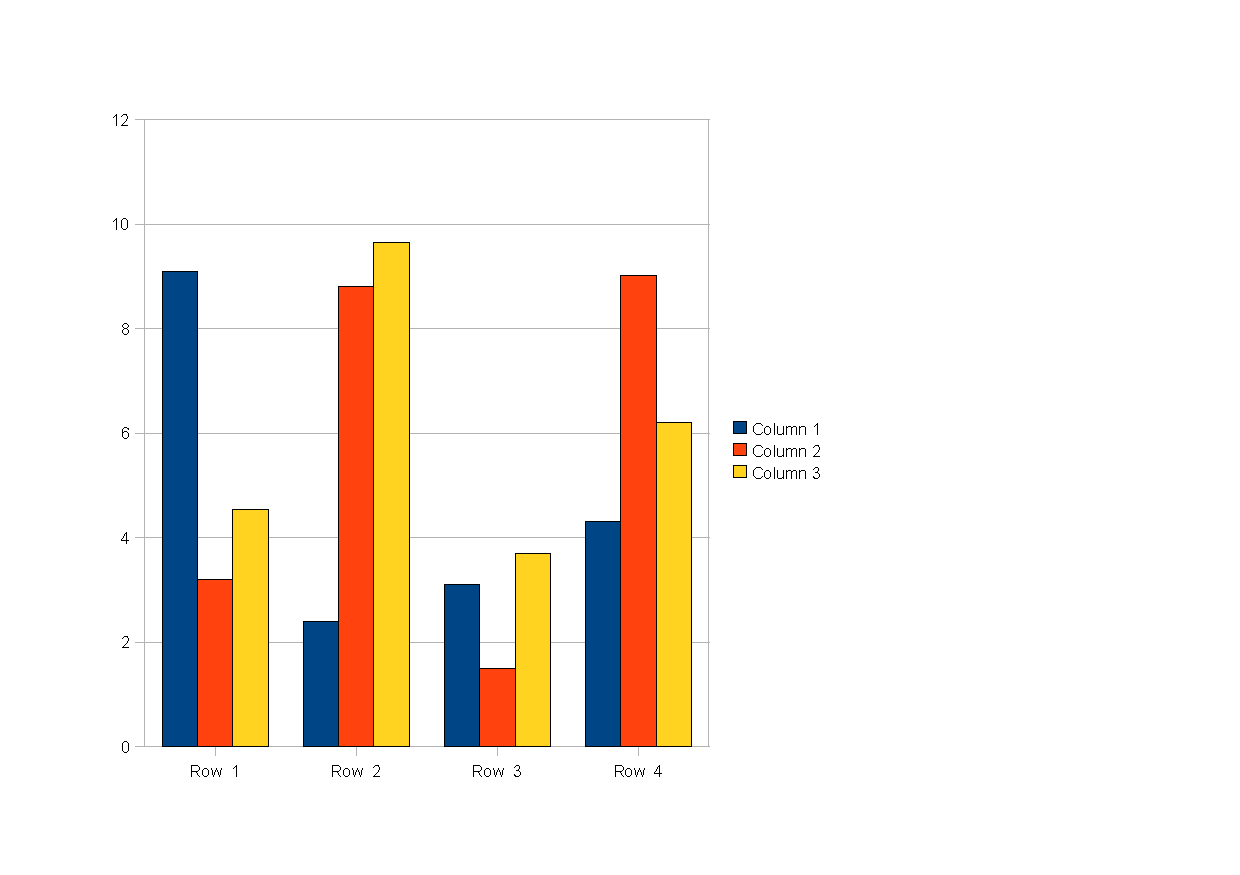
\includegraphics[width=\textwidth]{example_figure}
%  \caption{Example figure}\label{fig:example}
% \end{center}
%\end{figure}

\section*{Acknowledgements}
This research is supported by \ldots

% Bibliography
% ============
% You may either enter the bibliography manually, possibly making use of
% \label and \ref, or use BibTeX. The bibliography style is set
% automatically. You process the bibliography by BibTeX in the
% standard way and include it by:
\bibliography{mybib}

% If needed, add appendices here
%\section*{Appendix A: \ldots}

\correspondingaddress
\end{document}

% ======= Additional information ==========

% XeLaTeX
% =======
% The Prague Bulletin of Mathematical Linguistics is typeset by XeLaTeX.
% It is not required that you use XeLaTeX and the same fonts as will be used in the
% journal but it is better to do so if you could (so you have the same line and page breaks).
% If XeLaTeX is not available on your computer, you can even used standard LaTeX.

% Fonts
% =====
% In the printed version, fonts TeX Gyre Pagella (shipped with TeX Live 2008 or later)
% and DejaVu (http://dejavu.sourceforge.net/wiki/index.php/Main_Page)
% will be used. If you have XeLaTeX but not these fonts, you may need to install
% the fonts somewhere where your system (fontconfig) can find them. On Linux,
% try something like this:
% ln -s YOUR-TEXLIVE/2008/texmf-dist/fonts/opentype/public/ \
%  ${HOME}/.fonts/texlive-2008-otf-public
% If you are not able to install these fonts, you can instruct XeLaTeX
% to use its default fonts by \document[nofonts]{pbml}.

% If you want to typset examples in east Asian scripts, you have to use
% OpenType Unicode fonts that are freely redistributable and you have to
% include them with your article. If you must use nonfree or non-Unicode
% fonts, you must supply the examples as EPS or PDF with fonts embedded in
% the files (as the required subset).
% If encountering problems with the "bidi" package, contact pbml@ufal.mff.cuni.cz.

% Vector Graphics
% ===============
% The most portable graphics package is tikz which is a front end to pgf.
% This package is fully supported both in standard LaTeX and XeLaTeX.
% PSTricks is not currently available for XeLaTeX.

% Color Images
% ============
% The printed version of PBML does not allow color figures, so please convert
% all your figures to grayscale (or black&white), make sure they are legible
% and put them in a subdirectory called "grayscale".
% When specifying the filename in \includegraphics DO NOT include the
% subdirectory.
% Optionally, in addition to the default grayscale images, you can add also
% color versions of the figures to be published in the online version.
% Put such images in a subdirectory called "color" with the same filenames
% as the grayscale ones.
% To temporarily switch to color output and hypertext links, use
% \documentclass[color]{pbml}

% Including images and other files
% ===================================
% When loading the file you must use a relative path, never the full path.
% Load the images by \includegraphics
% and other files by \input, never use \include.
